
\subsubsection{Strukturplan}
\label{subsubsec:Strukturplan_Atmega}

In Abbildung \ref{fig:Softwareuebersicht_Atmega2560} wird aufgezeigt, wie die Software aufgebaut ist und welcher Teil der Software von welchen Libraries abhängig ist. Wie in Kapitel \ref{subsec:Software_Atmega2560} beschrieben kann die Software in folgende Teile gegliedert werden:
\begin{itemize}
\item Init/Main
\item User Application
\item API - Application-Programming-Interface
\item HAL - Hardware-Abstraction-Layer
\item Interfaces / Pins
\end{itemize}


\begin{figure}[H]
	\centering
	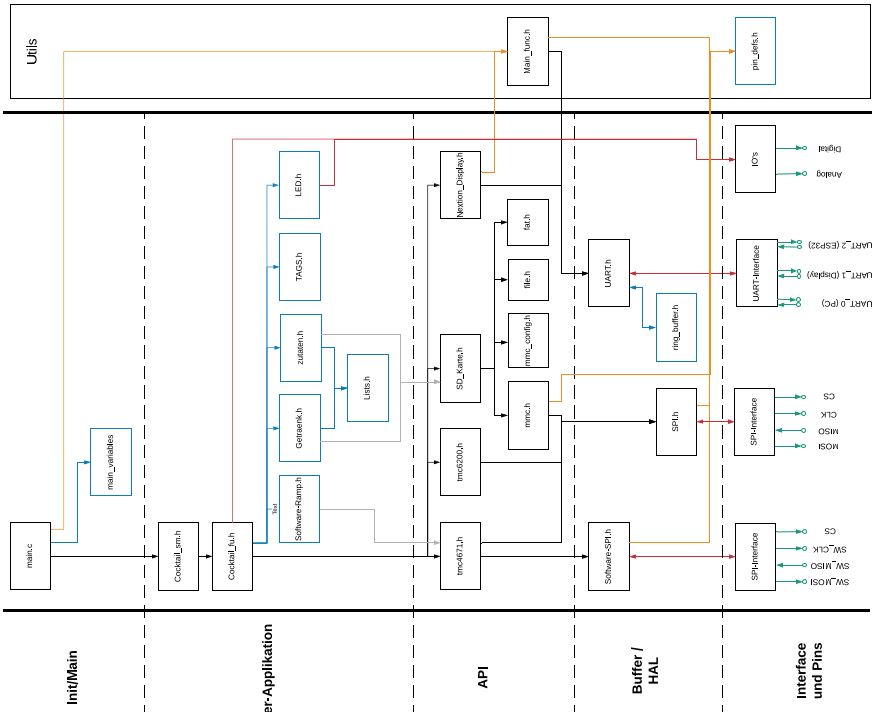
\includegraphics[angle = 270, width=\textwidth]{graphics/Softwareablauf}
	\caption{Softwareübersicht Mikrocontroller}
	\label{fig:Softwareuebersicht_Atmega2560}
\end{figure}